	\chapter{Conceptos Básicos en Sistemas Dinámicos}

\section{Espacios y Órbitas}

Consideremos un sistema dinámico discreto dado por un par $(M, f)$, donde $M$ puede ser un espacio topológico, una variedad diferenciable o un espacio medible, y $f: M \to M$ es una función (que será continua, diferenciable o medible, respectivamente). 

\begin{definicion}[Órbita futura y pasada]
	La \textbf{órbita futura} de $x \in M$ por $f$ se denota por $\mathcal{O}_f^+(x)$ y se define como el conjunto de iteraciones sucesivas:
	$$\mathcal{O}_f^+(x) = \{f^n(x) : n \in \mathbb{N} \cup \{0\}\}$$
	Si $f$ admite inversa (es decir, es biyectiva y $f^{-1}$ tiene las mismas propiedades de regularidad), definimos la \textbf{órbita pasada} de $x \in M$ como:
	$$\mathcal{O}_f^-(x) = \{f^{-n}(x) : n \in \mathbb{N} \cup \{0\}\}$$
	Y la \textbf{órbita total} como $\mathcal{O}_f(x) = \{f^n(x) : n \in \mathbb{Z}\}$.
\end{definicion}

\begin{ejemplo}
	Sea $f: \mathbb{R} \to \mathbb{R}$ dada por $f(x) = 2x$. 
	\begin{itemize}
		\item Para el punto $x = 0$, tenemos que $f(0) = 0$. Por lo tanto, su órbita futura y pasada trivializan en el origen: $\mathcal{O}_f^+(0) = \{0\}$.
		\item Para un punto $x_0 \neq 0$, por ejemplo $x_0 > 0$, las iteraciones sucesivas nos dan $f^n(x_0) = 2^n x_0$. Como se observa en el diagrama de telaraña de la Figura \ref{fig:orbita_2x}, al iterar la función, los puntos $x_1, x_2, \dots$ se alejan cada vez más, por lo que la órbita diverge hacia el infinito.
	\end{itemize}
\end{ejemplo}

\begin{figure}[htbp]
	\centering
	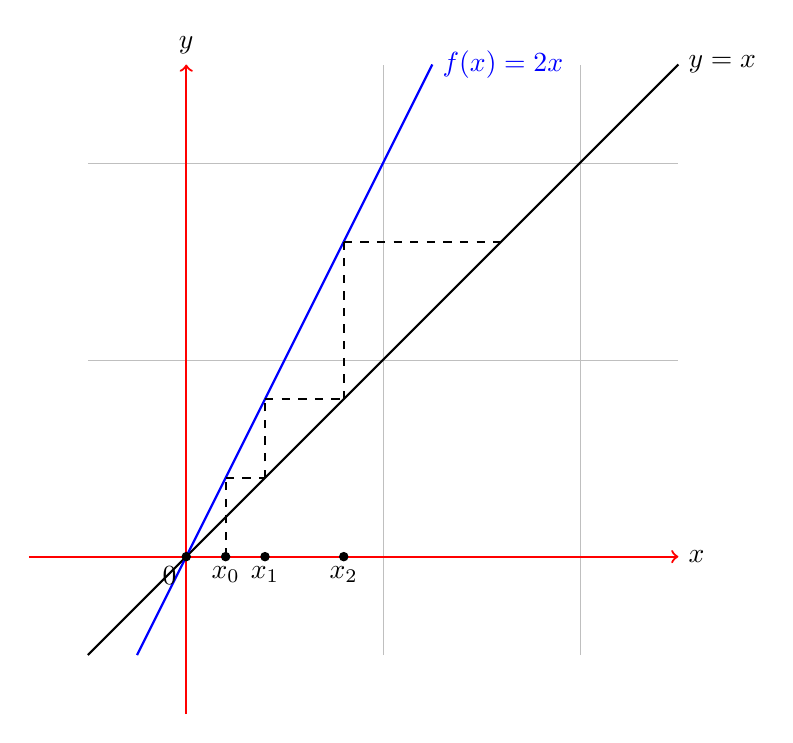
\begin{tikzpicture}[scale=2.5]
		% Cuadrícula de fondo
		\draw[lightgray, very thin] (-0.5,-0.5) grid (2.5,2.5);
		
		% Ejes
		\draw[thick, red, ->] (-0.8,0) -- (2.5,0) node[right, black] {$x$};
		\draw[thick, red, ->] (0,-0.8) -- (0,2.5) node[above, black] {$y$};
		
		% Recta y = x (identidad)
		\draw[thick, black] (-0.5,-0.5) -- (2.5,2.5) node[right] {$y=x$};
		
		% Función f(x) = 2x (en azul)
		\draw[thick, blue] (-0.25,-0.5) -- (1.25,2.5) node[right] {$f(x)=2x$};
		
		% Órbita (Diagrama de telaraña) partiendo de un x_0 pequeño
		\draw[dashed, black, thick] (0.2, 0) -- (0.2, 0.4); 
		\draw[dashed, black, thick] (0.2, 0.4) -- (0.4, 0.4); 
		\draw[dashed, black, thick] (0.4, 0.4) -- (0.4, 0.8); 
		\draw[dashed, black, thick] (0.4, 0.8) -- (0.8, 0.8); 
		\draw[dashed, black, thick] (0.8, 0.8) -- (0.8, 1.6); 
		\draw[dashed, black, thick] (0.8, 1.6) -- (1.6, 1.6); 
		
		% Puntos y etiquetas cuidadosamente espaciados
		\filldraw[black] (0,0) circle (0.6pt) node[below left] {$0$};
		\filldraw[black] (0.2,0) circle (0.6pt) node[below] {$x_0$};
		\filldraw[black] (0.4,0) circle (0.6pt) node[below] {$x_1$};
		\filldraw[black] (0.8,0) circle (0.6pt) node[below] {$x_2$};
	\end{tikzpicture}
	\caption{Gráfica de $f(x)=2x$ y diagrama de telaraña mostrando que la órbita $\mathcal{O}_f^+(x_0)$ diverge del origen.}
	\label{fig:orbita_2x}
\end{figure}

\section{Puntos Fijos y Periódicos}

\begin{definicion}[Puntos fijos y periódicos]
	El conjunto de los \textbf{puntos fijos} de $f$ se denota por $\text{Fix}(f)$ y se define por:
	$$\text{Fix}(f) = \{x \in M : f(x) = x\}$$
	El conjunto de los \textbf{puntos periódicos} de $f$ se denota por $\text{Per}(f)$ y se define por:
	$$\text{Per}(f) = \{x \in M : f^n(x) = x \text{ para algún } n \in \mathbb{N}\}$$
\end{definicion}

\begin{observacion}
	Se cumple que $\text{Fix}(f) \subset \text{Per}(f)$. En efecto, si tomamos $x \in \text{Fix}(f)$, por definición tenemos que $f(x) = x$. Esto significa que la condición de punto periódico $f^n(x) = x$ se satisface para el caso particular donde $n=1$. Por lo tanto, $x \in \text{Per}(f)$.
\end{observacion}

\begin{ejemplo}
	Considere la aplicación (conocida como el \textit{mapa tienda}) $f: [0,1] \to [0,1]$ definida por:
	$$ f(x) = \begin{cases} 
		2x & \text{si } 0 \le x < 1/2 \\ 
		2 - 2x & \text{si } 1/2 \le x \le 1 
	\end{cases} $$
	Halle explícitamente $\text{Fix}(f)$.
\end{ejemplo}

\begin{proof}[Solución]
	Para encontrar $\text{Fix}(f)$, resolvemos la ecuación $f(x)=x$ en ambos subintervalos:
	\begin{enumerate}
		\item Si $0 \le x < 1/2$, igualamos $2x = x \implies x = 0$.
		\item Si $1/2 \le x \le 1$, igualamos $2 - 2x = x \implies 3x = 2 \implies x = 2/3$.
	\end{enumerate}
	Por lo tanto, concluimos que $\text{Fix}(f) = \{0, 2/3\}$.
\end{proof}

\begin{figure}[htbp]
	\centering
	\begin{minipage}{0.31\textwidth}
		\centering
		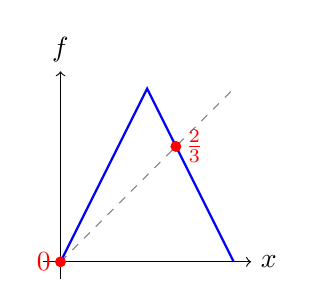
\begin{tikzpicture}[scale=2.2]
			\draw[->] (-0.1,0) -- (1.1,0) node[right] {$x$};
			\draw[->] (0,-0.1) -- (0,1.1) node[above] {$f$};
			\draw[dashed, gray] (0,0) -- (1,1);
			\draw[thick, blue] (0,0) -- (0.5,1) -- (1,0);
			\filldraw[red] (0,0) circle (0.8pt) node[left] {$0$};
			\filldraw[red] (0.666,0.666) circle (0.8pt) node[right] {$\frac{2}{3}$};
		\end{tikzpicture}
		\caption*{Iteración $f(x)$}
	\end{minipage}\hfill
	\begin{minipage}{0.31\textwidth}
		\centering
		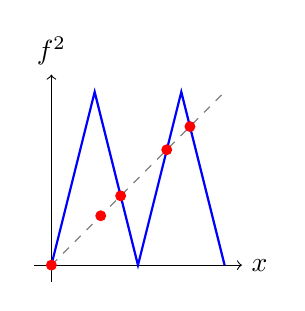
\begin{tikzpicture}[scale=2.2]
			\draw[->] (-0.1,0) -- (1.1,0) node[right] {$x$};
			\draw[->] (0,-0.1) -- (0,1.1) node[above] {$f^2$};
			\draw[dashed, gray] (0,0) -- (1,1);
			\draw[thick, blue] (0,0) -- (0.25,1) -- (0.5,0) -- (0.75,1) -- (1,0);
			\filldraw[red] (0,0) circle (0.8pt);
			\filldraw[red] (0.4,0.4) circle (0.8pt);
			\filldraw[red] (0.8,0.8) circle (0.8pt);
			\filldraw[red] (0.285,0.285) circle (0.8pt); 
			\filldraw[red] (0.666,0.666) circle (0.8pt);
		\end{tikzpicture}
		\caption*{Iteración $f^2(x)$}
	\end{minipage}\hfill
	\begin{minipage}{0.31\textwidth}
		\centering
		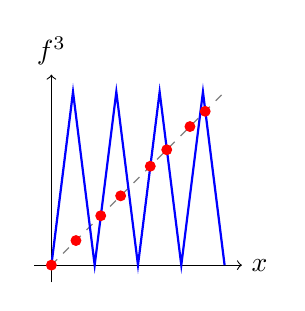
\begin{tikzpicture}[scale=2.2]
			\draw[->] (-0.1,0) -- (1.1,0) node[right] {$x$};
			\draw[->] (0,-0.1) -- (0,1.1) node[above] {$f^3$};
			\draw[dashed, gray] (0,0) -- (1,1);
			\draw[thick, blue] (0,0) -- (0.125,1) -- (0.25,0) -- (0.375,1) -- (0.5,0) -- (0.625,1) -- (0.75,0) -- (0.875,1) -- (1,0);
			% Solo marcando intersecciones referenciales
			\filldraw[red] (0,0) circle (0.8pt);
			\filldraw[red] (0.142,0.142) circle (0.8pt);
			\filldraw[red] (0.285,0.285) circle (0.8pt);
			\filldraw[red] (0.4,0.4) circle (0.8pt);
			\filldraw[red] (0.571,0.571) circle (0.8pt);
			\filldraw[red] (0.666,0.666) circle (0.8pt);
			\filldraw[red] (0.8,0.8) circle (0.8pt);
			\filldraw[red] (0.888,0.888) circle (0.8pt);
		\end{tikzpicture}
		\caption*{Iteración $f^3(x)$}
	\end{minipage}
	\caption{El mapa tienda y sus iteraciones sucesivas. Las intersecciones con $y=x$ (puntos rojos) revelan el crecimiento exponencial de los puntos periódicos.}
	\label{fig:mapa_tienda_iteraciones}
\end{figure}

\begin{ejercicio}
	Definamos $\text{Per}_n(f) = \{x \in M : f^n(x) = x\}$. Para el mapa tienda $f$ definido en el ejemplo anterior:
	\begin{enumerate}[a)]
		\item Halle explícitamente $\text{Per}_n(f)$.
		\item Muestre que $\overline{\text{Per}(f)} = [0,1]$.
		\item ¿Se cumple que $\text{Per}(f) = [0,1]$?
	\end{enumerate}
\end{ejercicio}

\begin{proof}[Solución]
	\textbf{a)} Podemos partir la función en 2 partes: $f_1(x) = 2x$ y $f_2(x) = 2 - 2x$. Las iteraciones de $f$ siguen un algoritmo constructivo donde, para calcular $f^n$, el intervalo se divide en $2^n$ partes iguales. En la Figura \ref{fig:algoritmo_f} observamos el árbol completo con el desglose hasta $f^3$, mostrando claramente la estructura de ramificación de este algoritmo.
	
	\begin{figure}[htbp]
		\centering
		% Usaremos resizebox por si la gráfica se sale ligeramente de los márgenes en algunas configuraciones, 
		% asegurando que el despliegue de las 8 ramas se vea impecable.
		\resizebox{\textwidth}{!}{
			\begin{tikzpicture}[
				box/.style={draw, thick, rounded corners, align=center, minimum width=2.5cm, minimum height=0.6cm},
				arrow/.style={-{Stealth}, thick, shorten >=2pt, shorten <=2pt}
				]
				% Nivel 1
				\node[box, text=blue, draw=blue] (f1) at (0, 2) {$f_1$};
				\node[box, text=blue, draw=blue] (f2) at (0, -2) {$f_2$};
				
				% Nivel 2
				\node[box] (f11) at (4, 3) {$f_1 \circ f_1$};
				\node[box] (f21) at (4, 1) {$f_2 \circ f_1$};
				\node[box] (f12) at (4, -1) {$f_1 \circ f_2$};
				\node[box] (f22) at (4, -3) {$f_2 \circ f_2$};
				
				% Nivel 3 (Completo y sin superposiciones)
				\node[box, text=red, draw=red] (f111) at (8.5, 3.5) {$f_1 \circ f_1 \circ f_1$};
				\node[box, text=red, draw=red] (f211) at (8.5, 2.5) {$f_2 \circ f_1 \circ f_1$};
				
				\node[box, text=red, draw=red] (f121) at (8.5, 1.5) {$f_1 \circ f_2 \circ f_1$};
				\node[box, text=red, draw=red] (f221) at (8.5, 0.5) {$f_2 \circ f_2 \circ f_1$};
				
				\node[box, text=red, draw=red] (f112) at (8.5, -0.5) {$f_1 \circ f_1 \circ f_2$};
				\node[box, text=red, draw=red] (f212) at (8.5, -1.5) {$f_2 \circ f_1 \circ f_2$};
				
				\node[box, text=red, draw=red] (f122) at (8.5, -2.5) {$f_1 \circ f_2 \circ f_2$};
				\node[box, text=red, draw=red] (f222) at (8.5, -3.5) {$f_2 \circ f_2 \circ f_2$};
				
				% Puntos suspensivos indicando la continuación del algoritmo
				\node[font=\bfseries\Huge] at (12, 0) {$\dots$};
				
				% Flechas Nivel 1 a 2
				\draw[arrow, blue] (f1.east) to[out=0, in=180] (f11.west);
				\draw[arrow, blue] (f1.east) to[out=0, in=180] (f21.west);
				\draw[arrow, blue] (f2.east) to[out=0, in=180] (f12.west);
				\draw[arrow, blue] (f2.east) to[out=0, in=180] (f22.west);
				
				% Flechas Nivel 2 a 3
				\draw[arrow, red] (f11.east) to[out=0, in=180] (f111.west);
				\draw[arrow, red] (f11.east) to[out=0, in=180] (f211.west);
				
				\draw[arrow, red] (f21.east) to[out=0, in=180] (f121.west);
				\draw[arrow, red] (f21.east) to[out=0, in=180] (f221.west);
				
				\draw[arrow, red] (f12.east) to[out=0, in=180] (f112.west);
				\draw[arrow, red] (f12.east) to[out=0, in=180] (f212.west);
				
				\draw[arrow, red] (f22.east) to[out=0, in=180] (f122.west);
				\draw[arrow, red] (f22.east) to[out=0, in=180] (f222.west);
				
				% Textos guía
				\node[font=\bfseries] at (4, 4.2) {$f^2$ (4 partes)};
				\node[font=\bfseries] at (8.5, 4.2) {$f^3$ (8 partes)};
			\end{tikzpicture}
		}
		\caption{Algoritmo de combinaciones ramificadas de $f_1$ y $f_2$ demostrando la expansión total hasta $f^3$.}
		\label{fig:algoritmo_f}
	\end{figure}
	
	Cada parte de $f^n$ se da por las combinaciones de $f_1$ y $f_2$ (es decir, composiciones de la forma $f_{j_n} \circ \dots \circ f_{j_1}$). Además, como tanto $f_1$ como $f_2$ son funciones lineales, la composición truncada en cada subintervalo es también una función lineal. Por ende, la solución de igualar esta composición truncada a la función identidad siempre nos dará a lo sumo un punto. Como consecuencia, $\text{Per}_n(f)$ tiene como máximo $2^n$ puntos periódicos distintos.
	
	\textbf{b)} Según el razonamiento algorítmico anterior, al dividir el intervalo $[0,1]$ en $2^n$ partes, sabemos que los puntos fijos de $f^n$ deben habitar cada uno de estos subintervalos. 
	Sean $x_0 \in (0,1)$ y $\epsilon > 0$ arbitrarios. Existe $N \in \mathbb{N}$ tal que $\frac{1}{2^N} < \epsilon$. Dividimos el intervalo en $2^N$ partes. Por ende, $x_0$ pertenece a algún subintervalo de longitud $\frac{1}{2^N}$. De esta manera, garantizamos que existe algún punto periódico $x$ cuya distancia a $x_0$ es como máximo $\frac{1}{2^N}$. 
	Luego, la distancia $|x - x_0| \le \frac{1}{2^N} < \epsilon$, por lo que $x \in V_\epsilon(x_0)$. Esto demuestra la densidad: $\overline{\text{Per}(f)} = [0,1]$.
	
	\textbf{c)} ¡No! Esto es incorrecto. Las composiciones truncadas de $f_1$ y $f_2$ tienen constantes racionales. Para algún $f^n_j$ en particular, tendrá esta regla de correspondencia: $f^n_j(x) = ax - b$, donde $a, b \in \mathbb{Q}$. El punto periódico es la solución a $ax - b = x$, de donde obtenemos $x = \frac{b}{a-1}$ (con $a \neq 1$). 
	Dado que $a,b \in \mathbb{Q}$, el punto periódico resultante será siempre un número racional. Como el intervalo $[0,1]$ contiene números irracionales, es imposible que $\text{Per}(f) = [0,1]$.
\end{proof}

\begin{ejemplo}
	Considere la rotación del círculo $S^1 \to S^1$, donde $S^1 = \{z \in \mathbb{C} : |z| = 1\}$. Definimos la aplicación $R_\theta(z) = z e^{2\pi i \theta}$, con un $\theta \in (0,1)$ fijo.
	Si evaluamos un ángulo racional, digamos $\theta = p/q \in \mathbb{Q}$, todos los puntos completarán ciclos exactos, por lo que es directo verificar que $\text{Per}(R_{p/q}) = S^1$. Esto se puede observar en la Figura \ref{fig:rotaciones}(a).
\end{ejemplo}

\begin{ejercicio}
	Para la aplicación $R_\theta: S^1 \to S^1$ definida anteriormente, demuestre que si $\theta \notin \mathbb{Q}$ (es irracional), entonces $\overline{\mathcal{O}^+_{R_\theta}(z)} = S^1$ para todo $z \in S^1$. (Ver visualización en la Figura \ref{fig:rotaciones}(b)).
\end{ejercicio}

\begin{figure}[htbp]
	\centering
	\begin{minipage}{0.45\textwidth}
		\centering
		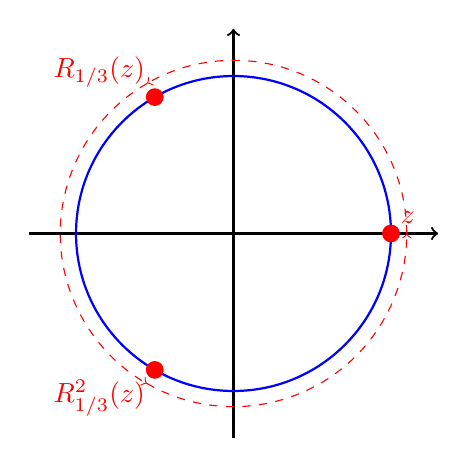
\begin{tikzpicture}[scale=2]
			\draw[thick, ->] (-1.3,0) -- (1.3,0);
			\draw[thick, ->] (0,-1.3) -- (0,1.3);
			\draw[thick, blue] (0,0) circle (1);
			
			\filldraw[red] (1,0) circle (1.5pt) node[above right] {$z$};
			\filldraw[red] (-0.5,0.866) circle (1.5pt) node[above left] {$R_{1/3}(z)$};
			\filldraw[red] (-0.5,-0.866) circle (1.5pt) node[below left] {$R_{1/3}^2(z)$};
			
			% Flechas de rotacion
			\draw[->, dashed, red] (1.1,0) arc (0:120:1.1);
			\draw[->, dashed, red] (-0.55,0.952) arc (120:240:1.1);
			\draw[->, dashed, red] (-0.55,-0.952) arc (240:360:1.1);
		\end{tikzpicture}
		\caption*{(a) $\theta = 1/3 \in \mathbb{Q}$}
	\end{minipage}\hfill
	\begin{minipage}{0.45\textwidth}
		\centering
		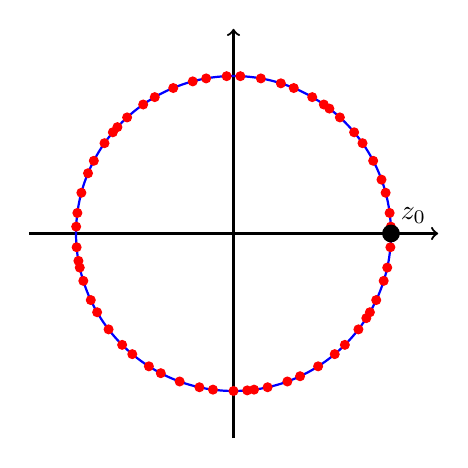
\begin{tikzpicture}[scale=2]
			\draw[thick, ->] (-1.3,0) -- (1.3,0);
			\draw[thick, ->] (0,-1.3) -- (0,1.3);
			\draw[thick, blue] (0,0) circle (1);
			
			% Bucle para generar densidad irracional
			\foreach \i in {1,...,60} {
				\filldraw[red] ({cos(\i*137.5)}, {sin(\i*137.5)}) circle (0.8pt);
			}
			\filldraw[black] (1,0) circle (1.5pt) node[above right] {$z_0$};
		\end{tikzpicture}
		\caption*{(b) $\theta \notin \mathbb{Q}$ (Denso)}
	\end{minipage}
	\caption{Dinámica de la rotación en $S^1$. Si $\theta$ es racional, la órbita es finita y periódica. Si $\theta$ es irracional, la órbita envuelve el círculo denso.}
	\label{fig:rotaciones}
\end{figure}

\begin{proof}
	En lugar de pensar en $R_\theta: S^1 \to S^1$, pensaremos en la dinámica de una manera equivalente. Consideremos la función $f: \mathbb{R}/\mathbb{Z} \to \mathbb{R}/\mathbb{Z}$ (que identificamos con el intervalo $[0,1)$) donde $f([x]) = [x+\theta] \pmod 1$.
	
	Tomemos un $\epsilon > 0$. Existe $N \in \mathbb{N}$ tal que $1/N < \epsilon$. De esta manera, dividimos el intervalo $[0,1)$ en $N$ piezas de igual longitud: $[0, 1/N), [1/N, 2/N), \dots, [(N-1)/N, 1)$.
	
	Ahora tomamos los primeros $N+1$ puntos de la órbita de cualquier $x$ fijo: $x, f(x), f^2(x), \dots, f^N(x)$. Por el Principio del Palomar, como tenemos $N+1$ puntos y solo $N$ piezas, existen al menos 2 puntos que se ubican en la misma pieza. Es decir, existen $j < k$ con $0 \le j < k \le N$ tales que $f^j(x)$ y $f^k(x)$ están en el mismo subintervalo.
	
	La distancia entre estos dos puntos es $\delta = d(f^k(x), f^j(x)) \le 1/N < \epsilon$. Notemos matemáticamente que la diferencia es:
	$$f^k(x) - f^j(x) = [x+k\theta] - [x+j\theta] = [(k-j)\theta] \pmod 1$$
	Sea $m = k-j$. La aplicación $f^m$ avanza de manera pequeñísima una distancia de $\delta$. Y como $\delta$ es menor a $\epsilon$ (la longitud de cualquier vecindad de tamaño $1/N$), entonces es imposible que la iteración salte alguna pieza. Finalmente, la órbita acabará cayendo en algún momento en cualquier pieza o vecindad a la que queramos llegar.
	
	Para regresar al círculo unitario, sea $T: S^1 \to \mathbb{R}/\mathbb{Z}$ dada por $T(e^{2\pi i x}) = [x]$. Se tiene la relación $T \circ R_\theta = f \circ T$. 
	Por ende, sea $z_0 \in S^1$ un punto fijo y un abierto $U \subset S^1$. Su imagen $T(U)$ es un abierto en $\mathbb{R}/\mathbb{Z}$. Por la densidad demostrada arriba, existe algún $r \in \mathbb{N}$ tal que $f^{mr}(T(z_0)) \in T(U)$. 
	Como $f^{mr} \circ T = T \circ R_\theta^{mr}$, deducimos que $T(R_\theta^{mr}(z_0)) \in T(U)$, lo que implica que $R_\theta^{mr}(z_0) \in U$. Así, la órbita intersecta cualquier abierto, demostrando que $\overline{\mathcal{O}^+_{R_\theta}(z)} = S^1$.
\end{proof}

\section{Conjuntos Límite}

\begin{definicion}[Conjuntos Límite $\omega$ y $\alpha$]
	Sea $f: M \to M$ una aplicación continua y $M$ un espacio topológico de Hausdorff y localmente compacto. El \textbf{conjunto $\omega$-límite} de $x$ por $f$, se denota por $\omega_f(x)$ y se define por:
	$$\omega_f(x) = \{y \in M : \exists \text{ sucesión } (n_k) \subseteq \mathbb{Z}^+ / f^{n_k}(x) \xrightarrow{k \to \infty} y\}$$
	Si $f$ es invertible, podemos definir el \textbf{conjunto $\alpha$-límite} de $x$ por $f$ como:
	$$\alpha_f(x) = \{y \in M : \exists \text{ sucesión } (n_k) \subseteq \mathbb{Z}^+ / f^{-n_k}(x) \xrightarrow{k \to \infty} y\}$$
\end{definicion}

\begin{ejemplo}
	Analicemos los conjuntos límite para algunas funciones:
	\begin{itemize}
		\item \textbf{Para $f(x)=2x$}: 
		Si $x \neq 0$, la órbita diverge a infinito, por lo que $\omega_f(x) = \emptyset$.
		Si $x = 0$, la órbita es fija, por lo que $\omega_f(0) = \{0\} = \alpha_f(0)$.
		Para el límite pasado con $x \neq 0$, $f^{-n}(x) = x/2^n \to 0$, por ende $\alpha_f(x) = \{0\}$.
		
		\item \textbf{Para la rotación $R_{1/3}$}:
		Sabemos que $\mathcal{O}_{R_{1/3}}^+(z) = \{z, R_{1/3}(z), R_{1/3}^2(z)\}$.
		Como las iteraciones son periódicas ($R_{1/3}^{3k}(z) = z$, $R_{1/3}^{3k+1}(z) = R_{1/3}(z)$, etc.), concluimos que $\omega_{R_{1/3}}(z) = \mathcal{O}_{R_{1/3}}^+(z)$ y por invertibilidad $\alpha_{R_{1/3}}(z) = \mathcal{O}_{R_{1/3}}^+(z)$.
	\end{itemize}
\end{ejemplo}

\begin{ejercicio}
	Si $p \in \text{Per}(f)$ con periodo $k \in \mathbb{Z}^+$. Demuestre que $\omega_f(p) = \mathcal{O}_f^+(p)$.
\end{ejercicio}
\begin{proof}[Solución]
	Como $f^k(p) = p$ y $f^i(p) \neq p$ para todo $1 \le i < k$, tenemos que la órbita es finita: $\mathcal{O}_f^+(p) = \{p, f(p), \dots, f^{k-1}(p)\}$. Es claro que $\mathcal{O}_f^+(p) \subseteq \omega_f(p)$.
	Ahora, si $x \in \omega_f(p)$, existe una sucesión $n_j \to \infty$ tal que $f^{n_j}(p) \to x$. Como la órbita $\mathcal{O}_f^+(p)$ es un conjunto discreto y finito, la única forma de que la sucesión converja a $x$ es que eventualmente sea constante e igual a $x$. Luego, $x \in \mathcal{O}_f^+(p)$.
\end{proof}

\begin{definicion}[Conjunto Invariante]
	Decimos que $A \subseteq M$ es invariante (para adelante) por $f: M \to M$ si $f(A) \subseteq A$.
\end{definicion}

\begin{ejemplo}
	Los conjuntos $\text{Fix}(f)$ y $\text{Per}(f)$ son invariantes.
	\begin{itemize}
		\item Para $\text{Fix}(f)$: Sea $x \in \text{Fix}(f) \implies f(x) = x \in \text{Fix}(f)$. Por ende $f(\text{Fix}(f)) \subseteq \text{Fix}(f)$. Además $x \in f(\text{Fix}(f))$ porque $\exists y \in \text{Fix}(f)$ tal que $f(y)=x$, de hecho $y=x$. Así, $f(\text{Fix}(f)) = \text{Fix}(f)$.
		\item Para $\text{Per}(f)$: Sea $x \in \text{Per}(f) \implies \exists y \in \text{Per}(f)$ tal que $f(x)=y$. Como $x$ es periódico, $\exists k \in \mathbb{Z}^+$ tal que $f^k(x)=x$. Evaluando: $f^k(y) = f^k(f(x)) = f(f(f^{k-1}(x))) = f(x) = y$. Entonces $y \in \text{Per}(f)$.
	\end{itemize}
\end{ejemplo}

\begin{proposicion}
	Si $M$ es un espacio topológico de Hausdorff y localmente compacto, entonces para todo $x \in M$, el conjunto $\omega_f(x)$ es cerrado e invariante por $f$ (es decir, $f(\omega_f(x)) = \omega_f(x)$).
\end{proposicion}

\begin{proof}
	Primero, demostramos que $\omega_f(x)$ es cerrado. Por definición, el conjunto puede escribirse equivalentemente como:
	$$\omega_f(x) = \bigcap_{k \ge 1} \overline{\{f^n(x) : n \ge k\}}$$
	Al ser la intersección arbitraria de conjuntos cerrados, $\omega_f(x)$ es cerrado (AF1).
	
	Para probar la invarianza (AF2), sea $y \in \omega_f(x)$. Existe una sucesión $n_k \to \infty$ tal que $f^{n_k}(x) \to y$. Por la continuidad de $f$, deducimos que $f(f^{n_k}(x)) \to f(y)$, lo cual se reescribe como $f^{n_k+1}(x) \to f(y)$. Puesto que la sucesión de índices $n_k+1$ también tiende a infinito, concluimos que $f(y) \in \omega_f(x)$. 
\end{proof}

\begin{definicion}[Conjunto Límite Global]
	Definimos las uniones de todos los conjuntos límite como:
	$$L_+(f) = \overline{\bigcup_{x \in M} \omega_f(x)}, \quad L_-(f) = \overline{\bigcup_{x \in M} \alpha_f(x)}$$
	El conjunto límite global de $f$ se denota por $L(f)$ y se define por $L(f) = L_+(f) \cup L_-(f)$.
\end{definicion}

\begin{observacion}
	Se cumple la cadena de inclusiones: $\text{Fix}(f) \subseteq \text{Per}(f) \subseteq L(f)$.
	\textbf{Demostración:} Sea $x \in \text{Per}(f)$ con periodo $m \in \mathbb{Z}^+$. Como demostramos anteriormente, $\omega_f(x) = \mathcal{O}_f^+(x) = \{x, f(x), \dots, f^{m-1}(x)\}$. Dado que $x \in \omega_f(x)$, entonces $x \in \bigcup_{y \in M} \omega_f(y) \subseteq L_+(f) \subseteq L(f)$.
\end{observacion}

\begin{observacion}
	Las inclusiones anteriores pueden ser estrictas: $\text{Fix}(f) \subsetneq \text{Per}(f) \subsetneq L(f)$.
	Por ejemplo, para la rotación irracional $f = R_{\sqrt{2}/2}$, no existen puntos fijos ni periódicos ($\text{Fix}(f) = \emptyset, \text{Per}(f) = \emptyset$). Sin embargo, como $\overline{\mathcal{O}_{R_{\sqrt{2}/2}}^+(z)} = S^1$, tenemos que $\omega_{R_{\sqrt{2}/2}}(z) = S^1$, lo que implica que $L(f) = S^1$.
\end{observacion}

\begin{ejercicio}
	Demuestre que $L(f)$ es invariante para adelante por $f$ (asumiendo $f \in C^0$).
\end{ejercicio}
\begin{proof}[Solución]
	Sea $y \in f(L(f))$. Sin pérdida de generalidad (trabajando con $L_+$), esto implica que $y = f(x)$ donde $x \in L_+(f) = \overline{\bigcup_{z \in M} \omega_f(z)}$.
	Entonces $f(x) \in f\left(\overline{\bigcup_{z \in M} \omega_f(z)}\right)$. Por continuidad, $f(\overline{A}) \subseteq \overline{f(A)}$, por lo que:
	$$f(x) \in \overline{f\left(\bigcup_{z \in M} \omega_f(z)\right)} \subseteq \overline{\bigcup_{z \in M} f(\omega_f(z))}$$
	Como $\omega_f(z)$ es invariante, $f(\omega_f(z)) \subseteq \omega_f(z)$, lo que nos da:
	$$\overline{\bigcup_{z \in M} f(\omega_f(z))} \subseteq \overline{\bigcup_{z \in M} \omega_f(z)} = L_+(f) \subseteq L(f)$$
	Por ende, $f(L(f)) \subseteq L(f)$.
\end{proof}

\section{Puntos No Errantes}

\begin{definicion}[Conjunto No Errante]
	Sea $M$ un espacio topológico de Hausdorff. Decimos que $x \in M$ es un \textbf{punto no errante} si para cualquier vecindad abierta $U$ de $x$ y para todo $N \ge 1$, existe un $n \ge N$ tal que:
	$$f^n(U) \cap U \neq \emptyset$$
	El conjunto de todos los puntos no errantes de $f$ se denota por $\Omega(f)$. De igual forma, el conjunto de puntos errantes es su complemento, $\Omega(f)^c$.
\end{definicion}

\begin{proposicion}
	Se cumplen las siguientes propiedades para $\Omega(f)$:
	\begin{enumerate}[i)]
		\item $\Omega(f)$ es cerrado.
		\item $f(\Omega(f)) \subseteq \Omega(f)$ asumiendo que $f \in C^0$.
		\item Si $f$ es homeomorfismo $\implies f(\Omega(f)) = \Omega(f)$.
	\end{enumerate}
\end{proposicion}

\begin{proof}
	\textbf{i)} Demostraremos que el complemento $\Omega(f)^c$ es abierto en $M$. 
	Sea $x \in \Omega(f)^c$. Existe una vecindad abierta $U \subseteq M$ de $x$ tal que $f^n(U) \cap U = \emptyset$ para todo $n \in \mathbb{Z}^+$. Luego, cualquier elemento dentro de $U$ también cumple esta condición de punto errante, por ende $U \subseteq \Omega(f)^c$, probando que es abierto.
	
	\textbf{ii)} Si $y \in f(\Omega(f))$, existe $x \in \Omega(f)$ tal que $f(x) = y$. Sea $V_y$ una vecindad arbitraria de $y$. Como $f$ es continua, $f^{-1}(V_y)$ es una vecindad abierta de $x$.
	Dado que $x \in \Omega(f)$, existe $n \in \mathbb{Z}^+$ tal que $f^n(f^{-1}(V_y)) \cap f^{-1}(V_y) \neq \emptyset$.
	Esto implica que existe un elemento $z$ que pertenece a ambos conjuntos. Si $z \in f^{-1}(V_y)$, entonces $f(z) \in V_y$. Por otro lado, si $z \in f^n(f^{-1}(V_y))$, entonces $z = f^n(w)$ para algún $w \in f^{-1}(V_y)$. Evaluando $f$, tenemos $f(z) = f^{n+1}(w) = f^n(f(w))$. Como $f(w) \in V_y$, entonces $f(z) \in f^n(V_y)$.
	Por lo tanto, $f(z) \in f^n(V_y) \cap V_y \neq \emptyset$, demostrando que $y \in \Omega(f)$.
	
	\textbf{iii)} (Ejercicio) Si $f$ es homeomorfismo, aplicamos ii) a la función inversa: $f^{-1} \in C^0 \implies f^{-1}(\Omega(f)) \subseteq \Omega(f)$. Aplicando $f$ a ambos lados, obtenemos $\Omega(f) \subseteq f(\Omega(f))$. Combinando esto con la parte ii), concluimos que $f(\Omega(f)) = \Omega(f)$.
\end{proof}

\begin{proposicion}
	Se cumple la inclusión: $L(f) \subseteq \Omega(f)$.
\end{proposicion}

\begin{proof}
	Recordemos que $L(f) = L_+(f) \cup L_-(f)$. Trabajaremos con $y \in L_+(f) = \overline{\bigcup_{x \in M} \omega_f(x)}$ (el análisis para $L_-$ es análogo). Dividiremos la prueba en dos casos:
	
	\textbf{Caso 1:} $y \in \bigcup_{x \in M} \omega_f(x)$. Esto significa que $y \in \omega_f(x)$ para algún $x \in M$. Luego existe una sucesión $(n_k) \subseteq \mathbb{Z}^+$ tal que $f^{n_k}(x) \to y$. Sea $U$ una vecindad de $y$. Existen índices $m > n > 0$ tales que $f^n(x), f^m(x) \in U$.
	Así, $f^{m-n}(f^n(x)) = f^m(x) \in U$. Como $f^n(x) \in U$, entonces $f^{m-n}(U) \cap U \neq \emptyset$, por lo que $y \in \Omega(f)$.
	
	\textbf{Caso 2:} $y \in \partial\left(\bigcup_{x \in M} \omega_f(x)\right)$. Sea $U$ una vecindad de $y$. Entonces, $U \cap \left(\bigcup_{x \in M} \omega_f(x)\right) \neq \emptyset$.
	Esto implica que $U \cap \omega_f(x) \neq \emptyset$ para algún $x \in M$. Sea $z \in U \cap \omega_f(x)$. Como $z \in \omega_f(x)$, por el Caso 1 sabemos que $z \in \Omega(f)$. Dado que $U$ es una vecindad de $z$, entonces $f^k(U) \cap U \neq \emptyset$ para algún $k \in \mathbb{Z}^+$. Al ser $U$ una vecindad arbitraria de $y$, se concluye que $y \in \Omega(f)$.
\end{proof}

\begin{ejercicio}
	Halle $\Omega(f)$ para las siguientes aplicaciones:
	\begin{enumerate}[a)]
		\item $f(x)=2x$ en $\mathbb{R}$
		\item $f(z)=R_{1/3}(z)$ en $S^1$
		\item $f(z)=R_{\sqrt{3}/3}(z)$ en $S^1$
		\item $f(x) = \begin{cases} 2x & : 0 \le x < 1/2 \\ 2-2x & : 1/2 \le x \le 1 \end{cases}$ en $[0,1]$
	\end{enumerate}
\end{ejercicio}
\begin{proof}[Solución]
	\textbf{a)} Es claro que $0 \in \Omega(f)$. Supongamos por el absurdo que existe un $x_0 \neq 0$ tal que $x_0 \in \Omega(f)$. Sin pérdida de generalidad, asumamos $x_0 > 0$. Sea el abierto $U = (3x_0/4, 5x_0/4)$.
	Entonces, sus iteraciones son de la forma $f^n(U) = (2^n \cdot 3x_0/4, 2^n \cdot 5x_0/4)$. Para $n \in \mathbb{Z}^+$, se tiene que $2^n \ge 2$. Por lo tanto, el extremo inferior de $f^n(U)$ es $\frac{3 \cdot 2^n}{4} x_0 \ge \frac{6}{4} x_0 > \frac{5}{4} x_0$. 
	Luego, $f^n(U) \cap U = \emptyset$ para todo $n \in \mathbb{Z}^+$, lo cual contradice que $x_0 \in \Omega(f)$. Así, $\Omega(f) = \{0\}$.
	
	\textbf{b)} Sabemos que todos sus puntos son periódicos. Por ende, para todo $x \in S^1$ y cualquier vecindad $U_x$, se cumple que $f^q(U_x) \supseteq f^q(x) = x \in U_x$ para algún $q \in \mathbb{N}$ (en este caso $q=3$). Por tanto, $f^q(U_x) \cap U_x \neq \emptyset \implies \Omega(f) = S^1$.
	
	\textbf{c)} Como $\theta = \sqrt{3}/3 \notin \mathbb{Q}$, probamos antes que $S^1 = \overline{\mathcal{O}_f^+(x)}$ para todo $x \in S^1$. Es decir, para toda vecindad $U_x$ existe $f^n(x) \in U_x$ y además $f^n(x) \in f^n(U_x)$. Esto asegura la intersección, por lo que $\Omega(f) = S^1$. (También se pudieron resolver fácilmente sabiendo que $\omega_f(x) = S^1$ para todo $x \in S^1$ y aplicando el Teorema de inclusión $L(f) \subseteq \Omega(f)$).
	
	\textbf{d)} Sabemos que para el mapa tienda $\overline{\text{Per}(f)} = [0,1]$. Sea $x \in [0,1]$. Para cualquier vecindad $U_x$, existe por densidad un punto $y \in \text{Per}(f)$ tal que $y \in U_x$. Al ser periódico, existe $n \in \mathbb{N}$ tal que $f^n(y) = y$.
	Luego, $y \in f^n(U_x)$ y también $y \in U_x$, de modo que $U_x \cap f^n(U_x) \neq \emptyset$. Así, $\Omega(f) = [0,1]$.
\end{proof}